\documentclass[10pt, a4paper]{article}

% Formatting
\usepackage{ctex}
\usepackage[margin=1in]{geometry}
\usepackage[titletoc,title]{appendix}

\usepackage[colorlinks,linkcolor=red]{hyperref}
\usepackage{amsmath,amsfonts,amssymb,mathtools}


\usepackage{graphicx,float}
\usepackage{xcolor}

\usepackage[ruled,vlined]{algorithm2e}
\usepackage{algorithmic}


\everymath{\displaystyle}


\usepackage{biblatex}
\addbibresource{references.bib}

% Title content
\title{数理统计学习笔记6-7}
\author{慕弋云子}
\date{November 1, 2020}

\begin{document}
\setcounter{section}{5}
\maketitle

写这些东西主要是为了:
\begin{enumerate}
    \item 对于期末突击的同学们,可以迅速把握考点和做题技巧。
    \item 对于保研的同学、或者已经忘了概统内容甚至完全没学过的同学,这是一份很好的补充材料。
    \item 对于历年新生,可以做到不必听课,独立阅读文档并认真完成老师留的作业,就可以很好地完成数理统计的学习。
\end{enumerate}

阅读本文前你需要知道:
\begin{enumerate}
    \item 本人是2020级孙海燕老师班的学生,首先必须声明的是,孙老师讲得挺好的,对于许多概念有着深厚的理解和把握,授课思路也很清晰,但大抵是要照顾各种程度的学生,所以进度对于我这样的考研学生就显得有些“食之无味,弃之可惜”。于是,我便解锁了边听课边写作业的操作,争取每周形成此文,带领大家巩固每周的内容并更好地完成作业。
    \item 数理统计本身的知识内容就有很强的抽象性,配合北航这形式化的教材,自学起来实在困难。所以我们不如找一个生动形象、轻松诙谐的方式,来共同完成一些概念的学习。在这个过程中可能不那么严谨,但会更加直观。
    \item 本文内容都是基于孙老师课堂内容及所布置作业,每一大节对应每节课的作业。对于本文未提及的知识点和习题类型,学有余力者可自行学习;本文内容亦不对诸位读者的考试成绩负责,还望知悉。
\end{enumerate}\par

此外,本人对于latex的使用略有生疏,以及对于数理统计知识的掌握难免有疏漏之处,还望见谅。如对本文内容有任何问题,欢迎私信或发邮件至:gt3115a@163.com。\par
另附本文GitHub Repo的地址,在这里你可以找到之前或之后的内容,不会迷路:\url{www.github.com/Muyiyunzi/ShuLiTongJi_BUAA}

\section{UMVUE}
作业内容参考:2.29、2.32、2.35、2.36\par
UMVUE指“一致最小方差无偏估计”(\textbf{U}niformly \textbf{M}inimum \textbf{V}ariance \textbf{U}nbiased \textbf{E}stimate),在上节内容中说过,如果说之前是“暴风雨前的宁静”,那么现在可能是“暴风雨夹雪”,可以说从本节内容开始难度陡增(尤其对于考研的同学)。\par
所以本次内容的首要目的是掌握做题的套路,其次就是尽量理解为什么这样做,或者至少能把握到我们在干一件什么样的事情,我认为这就够了。事实上在笔者查阅了陈希孺老师、茆诗松老师等人的书籍文献后仍然对一些概念理解得不好,所以我认为我也做不到讲述得完全严谨,但可以做到尽量生动有趣,如有任何谬误和理解偏差,也欢迎各位讨论与指正。\par

\subsection{引入:德国坦克问题}

 UMVUE的概念实在生涩,以及看这个名字就好像很吓人的样子,对萌新实在不够友好,所以我们以一个有趣的例子来引入这个问题。\\\par
\textbf{一个有趣的栗子.}(德国坦克问题,German Tank Problem)这个问题源自于二战。现在试想你是英国军队的指挥官。情报人员得知,德国人生产某一批次坦克时,会对每一辆坦克进行标号,而且这个编号是从1开始一个一个往后数的。在某次作战中,你的部队缴获了德国某同一批次的坦克两辆,分别印着编号为8号和10号。那么请问指挥官,这一批次德国人最可能生产了多少辆坦克?\\\par
现在我们把这个问题做形式化的建模:假设观察到的坦克序号来源于一个离散均匀分布$\{1,2, \ldots, N\}$,并且已经观察到的$k$个坦克(无重复)的最大序号是$m$,那么如何估计总数$N$。对应本例子就是:如果观察到了8号坦克和10号坦克,那么坦克的总数最可能是多少?\par
稍加思考之后,你一拍脑子,发现这不就是个最大似然估计问题吗,我学过啊。于是你开始了一通计算,最终计算出了N的最大似然估计居然就是10。如果你把这个事儿跟总指挥一讲,那我估计你这个指挥官的最大似然也会是“被开除”——缴获了八号和十号坦克,你告诉我德国人最可能生产十辆坦克??不过这虽然很反直观,但仔细一想却很好理解,这里给两种方式:\\\par
1.就硬算。求解N的最大似然,那就写似然函数呗$L=\frac{C^2_2}{C^2_N}=\frac{2}{N(N-1)}$,然后让对数似然函数对$N$求导得到$\frac{d\ln{L} }{dN}=-\frac{1}{N}-\frac{1}{N-1}$,而$N$事实上是大于等于$10$的,也就是说偏导恒负,所以$N$的最大似然是其可取范围内的最小值,也即$10$。\par
2.理解。你的$N$越大(基数越大),观察到$8$号和$10$号(取到8号球和10号球)的概率就越小。所以$N$当然是越小越好了,那么只能就是$10$了呗。兄弟萌把公屏打在李姐上。\\\par
所以,这时候该咋办呢?这就引入了我们的“一致最小方差无偏估计”,也就是说,我们希望它又是无偏估计,又是方差最小的,是最好的那个估计,但同时也必须要让模型满足一些条件才能得到。也因此,对UMVUE的求解通常很困难、结果也很复杂,然而诸君不必担心,求解也是有规可循的。\par
最终我们求出UMVUE的结果是14,这里具体的求解过程大家不必在意。如果实在想探究可以点击这个知乎链接:\href{https://zhuanlan.zhihu.com/p/158085371}{从中山大学王晓玮事件到德国坦克问题},但我认为在这个例子中UMVUE退化为了矩估计,并不能很好地体现其伟大和套路,所以真看的话图一乐就行了。\par
到此我们完成了对UMVUE的引入,如果时间紧张只想会做题,建议学习完下一节的“吃灰挖土”后直接跳到6.5、6.6节。

\subsection{完备充分统计量与“吃灰挖土”}

在讲UMVUE的这堆定理以及什么是“吃灰挖土”之前,我们有必要复习一下什么是\textbf{无偏估计}与\textbf{充分统计量}。\par
无偏估计很简单,即某个统计量$S$的数学期望$E(S)$正好等于我们要估计的参数$\theta$的函数$\varphi(\theta)$。注意无偏估计不一定存在,通常来讲也不唯一,所以这里通常会有一个更优问题:如果我们考虑两个无偏估计谁更优,就去求他们的方差,谁的方差比较小谁就更优,这一点也是比较好想象的。\par
至于充分统计量这个比较久远的概念,具体的定义大家可以翻看上一篇学习笔记,我在这里给一个更加直观生动的理解\footnote{\href{https://www.zhihu.com/question/41367707/answer/572628701}{求大神给解释解释充分统计量啊?}}:如果你在实验室三天三夜不吃不喝(请勿模仿)终于做出了足量的实验数据,几百张纸,带着满满的成就感,你终于可以睡个好觉了。然后第二天起来发现,这堆数据被狗吃了——这个时候假如你的数据满足正态分布,且你已经提前把这些数据的均值和方差记录在另外一张纸上了,那你的狗也没坏了什么大事,因为这两个充分统计量包含了这些数据的所有有用信息。我们可以把它们轻松还原出来,而这就是充分统计量的意义,即关于参数或者分布的此类有用\textbf{信息}都被包含在充分统计量里面了,一旦充分统计量确定,参数再怎么折腾也影响不了分布。\par
而我们寻找充分统计量的方式是求联合分布函数,然后使用\textbf{因子分解定理}找出$g(\theta)$、$h(x_1,\dots,x_n)$和$T(x_1,\dots,x_n)$,从而解出充分统计量$T$。\par
我们知道,充分统计量也经常是不唯一的,这时候我们就很贪,怎样的充分统计量是更好,或者说更「完备」的呢?(果然人类的进步源于贪心和懒惰hhh)\par
这里要给出一系列概念,请跟紧。\par
首先是\textbf{分布族}:我们在这里姑且认为一个概率密度函数可以代表一个分布族,最简单的比如二项分布、正态分布这些也都可以叫做一个分布族;\par
其次是\textbf{完备分布族}:如果我们对分布族$\phi(x,\theta)$(控制分布族的参数为$\theta$,自变量为$x$)做积分$\int \phi(x, \theta) d x$,注意这个积分很像数学期望,但是里边没有$x$,而是单纯地对概率密度积分,如果这个积分等于0,我们就能够推出$\phi(x, \theta)=0$的话,那么我们就称这个分布族为完备分布族。举例来说,$N\left(0, \sigma^{2}\right)$就是一个不完备分布族,因为无论你$\sigma$怎么变,概率密度函数总是对称的,积分总是为0。\par
然后是\textbf{完备统计量}:如果统计量「诱导」(大致理解为还原出来)的分布族是完备分布族,那么我们就称这个统计量为完备统计量。比如说上面这个例子中$T=\sum x_i$就是不完备统计量,然而$T=\sum {x_i} ^2$就是完备统计量了(因为平方之后分布族就不关于$y$轴对称了)。\par
那么对于\textbf{完备充分统计量}的求解,就要涉及指数族分布(或称指数型分布族)了,你可以把它看作是因子分解定理与完备统计量的一种结合,对于其具体定义不做展开,但总之都是通过“吃灰挖土”法来求解的。因为其要找出四个函数$c(\theta)$、$h(x_1,\dots,x_n)$、$w(\theta)$、$T(x_1,\dots,x_n)$,而$chwT$的首字母对应着很应双十一景的“吃灰挖土”,我便以此进行记忆,也算是分享给大家一个记忆方法,别无长物。\par
具体地,在我们求解完概率密度函数$p(x_1,\dots,x_n;\theta)$后,如果我们能将其分解为:
\begin{center}
   $p(x_1,\dots,x_n;\theta)=c(\theta)h(x_1,\dots,x_n)\exp\left\{w(\theta)T(x_1,\dots,x_n)\right\}$ 
\end{center}
的话,\textbf{并且}$w(\theta)$的值域有内点,则此时的$T(x_1,\dots,x_n)$即为\textbf{完备充分统计量}。\par
举个例子大家就明白了。比如我们现在求出联合密度函数为
\begin{center}
    $p(x_1,\dots,x_n;\theta)=\frac{1}{\theta ^n} \exp\{-\frac{1}{\theta} \sum_{i=1}^{n} x_i\} I_{\{x_{(1)} > 0\}} (x_1,\dots,x_n)$,$\theta>0$
 \end{center}

那么这个时候对应的“吃灰挖土”即为:$c(\theta)=\frac{1}{\theta ^n}$,$h(x_1,\dots,x_n)=I_{\{x_{(1)} > 0\}} (x_1,\dots,x_n)$,$w(\theta)=-\frac{1}{\theta}$,$T(x_1,\dots,x_n)=\sum_{i=1}^{n} x_i$。如果你对如何求充分统计量掌握的比较好,这一部分你应该接受起来会很快。\par

然后我们看$w(\theta)$和内点的概念:所谓值域有内点,就是存在一个内点,其邻域包含在值域内。比如$(0,10)$这个值域有内点,但0和10显然不是内点。\par

显然内点这东西很难没有,大家做题的时候\textbf{默认值域总是有内点}就行了。比如这里我们就应该说:$w(\theta)=-\frac{1}{\theta}$的值域是$(-\infty,0)$($\theta>0$),有内点(无脑写有就行了)。

在这里多强调一句,无论你使用哪种方法求解UMVUE,这一步都是必须要做的,如果到时候要考,这也应该是一个绝对的采分点。

\subsection{Rao-Blackwell定理}
我们再接着回过头来看UMVUE。建立在充分统计量的基础上(目前还没有完备什么事儿),Rao-Blackwell定理为我们提供了寻找UMVUE的一条思路。我们说过,UMVUE是那个方差最小的无偏估计,找到一个无偏估计很简单(如果忘了可以翻看上一次的内容),但是找到方差最小的怎么找?如果说这个寻找的过程是大海捞针,那么Rao-Blackwell定理揭示了,我们朝着一个什么样的方向去寻找,更能找到这个针。\par
在上一节内容中我偷偷地将「信息」加了粗,就是表明,这个“更可能的方向”必须要有「信息」的加持,所以我相信你也想到了,\textbf{如果我们对无偏估计施加以充分统计量的信息,这个无偏估计就会变得更好},这就是Rao-Blackwell定理在论证的事情。这里我就不再给出形式化的表述了(书上都有),而尝试给出更简略的表示。\par
\subsubsection*{Theorem 1 (Rao-Blackwell定理)}
若$S(x)$是充分统计量,$\varphi(x)$是$q(\theta)$方差有限的无偏估计,此时我们令$T(x)=E_\theta [\varphi(x) \mid S(x)]$,即给定$S(x)$后$\varphi(x)$的数学期望,为一新的统计量,则$T(x)$\textbf{也是}$q(\theta)$一个方差有限的\textbf{无偏估计},并且对于一切$\theta$都会有
\begin{center}
    $Var_\theta (T(x)) \leq Var_\theta (\varphi(x))$ 
\end{center}
当且仅当$T(x) = \varphi(x)$时(原文为依概率收敛到1,这里可以简单理解为等于)成立。\\\par

所以实际上Rao-Blackwell可以简洁地总结为两点:
\begin{enumerate}
    \item 对一个无偏估计,给定充分统计量求其期望,得到新的无偏估计,可以「优化」这个无偏估计。
    \item 只能给出一个更好的方向,但却不能保证找到针。(可以从收敛的角度理解)
\end{enumerate}

至于此定理的证明涉及测度论等内容,不做展开了(说的就跟之后哪个定理我能证一样,下同不证)。

\subsection{Lehmann-Scheffe定理}
如果说Rao-Blackwell论证了一个更好的方向去找针,那么Lehmann-Scheffe则巧妙地将「完备」这个东西引入了进来,并论证了在加持“完备充分统计量”这个信息的时候,无偏估计会直接质变为UMVUE。由于书上统一是用的「完全」这个词,所以我们尽量都说完全充分统计量,而在单独讨论完备这个概念的使用完备,这俩其实是一个东西哈。\par

定理的内容也比较质朴,其实直接看书上形式化的表述你会发现甚至能看懂,但为了尊重一下这个伟大的定理我还是单把它列出来吧。\par

\subsubsection*{Theorem 2 (Lehmann-Scheffe定理)}
若$S(x)$是完全充分统计量,$\varphi(x)$是$q(\theta)$无偏估计,类似地令$T(x)=E_\theta [\varphi(x) \mid S(x)]$,那么$T(x)$是$q(\theta)$唯一的UMVUE。\\\par
形象地理解,Rao-Blackwell是对信息进行了压缩,为我们提供了更好的方向,就好比说“钓鱼岛是中国的,大家朝着中国海域行驶应该就能找到钓鱼岛,但具体哪个岛是钓鱼岛我就不知道了”;那么Lehmann-Scheffe定理就好像在告诉我们“钓鱼岛位于北纬25°44.6′,东经123°28.4′,不管大家现在在哪儿,往这个坐标开就到钓鱼岛了”。这就是信息量差异带来的结果,对比并结合Rao-Blackwell定理我们可以大致看出,“完备”导致了唯一性(信息量越大就越精确),“充分”导致了最优性(信息量大并不意味着无偏,只有是充分统计量的情况下,这种优化才是保证无偏的)。\par

所以说Lehmann-Scheffe定理是Rao-Blackwell定理的一种延展,具体证明也是通过Rao-Blackwell定理及期望Jensen不等式等内容,在此不做展开。\par
而Lehmann-Scheffe定理之所以伟大,就是在于它甚至提供了两种方式来寻找UMVUE:
\begin{enumerate}
    \setcounter{enumi}{-1} 
    \item 无论是哪种方式,都要先找到完全充分统计量。
    \item 方式一就是找到一个无偏估计,随后计算条件期望$E_\theta [\varphi(x) \mid S(x)]$,这算是顺着Lehmann-Scheffe的定理表述找到UMVUE。
    \item 方式二则逆着来,如果完全充分统计量是无偏估计(给了坐标而且还是钓鱼岛),那这事儿就结了对吧;但如果完全充分统计量不是无偏估计,我们可以找一个它\textbf{的函数}是无偏估计,这样也能解决问题(比如你先到某某坐标,再西行xxx~km,这样也能唯一地找到钓鱼岛)。
\end{enumerate} \par
方式二的函数可以很复杂,开根号什么的都可以,但要注意对一个统计量开根号,其期望可不一定开根号,所以方式二有的时候会求的很艰辛,比如求出来期望差个根号,但实际对统计量开个根号以后再求期望还要修正一堆系数,往往还要会到Gamma分布中再求积分,我吐槽的是哪道题大家应该都知道了吧……\par
具体地,我们进入下两节来总结求解步骤。

\subsection{条件期望法求UVMUE}
首先对条件期望法求解步骤做一个总结:
\begin{enumerate}
    \item 首先进行“吃灰挖土”分解,无脑有内点,找到完全充分统计量。
    \item 找到一个无偏估计$\varphi(x)$,一般都是直接瞪出来的。
    \item 求条件期望$E_\theta [\varphi(x) \mid S(x)]$(其中$S(x)$为完全充分统计量,一般用$t$表示),求解时将$t$看做一个整体不要拆开,将期望看作是条件概率,将其对应地展开为两个概率的比值,并计算即可。
    \item 求解完成后,将具体的完全充分统计量替换t,即可得到UMVUE。
\end{enumerate} \par
使用此方法,我认为有两点需要稍加关注:
\begin{enumerate}
    \item 因为涉及到概率计算,所以需要注意\textbf{完全充分统计量}的取值范围,在某些情况下概率应该是0,对应地要分类讨论,最后结论时再“分久必合”。
    \item 再具体计算概率时,有时需要考虑分布族的可加性,比如泊松分布、两点分布等,但一般都是可加的,如果分析不清楚就回归到中心极限定理再做分析。
\end{enumerate} \par
总之,对于此方法的使用基本就是严格按照Lehmann-Scheffe定理的表述来的,应该是用起来最得心应手的,往往适用于那些泊松、几何、两点等非常易于瞪出来无偏估计的分布问题。
\subsection{寻找函数法求UMVUE}
同样先对寻找函数法求解步骤做一个总结,这个名字是我自己起的,似乎也有叫直接法的:
\begin{enumerate}
    \item 首先还是进行“吃灰挖土”分解,无脑有内点,找到完全充分统计量$T$。
    \item 求$T$的期望,要是正好等于待估计参数函数,那问题解决。
    \item 接下来就要吃一些技巧了。我个人认为是,对比$T$的期望和待估计参数函数的「量级」,做出相应的变换再求期望。
    \item 随后修正这个期望,一般来讲就是常数系数,但如果还是差量级,就继续做变换。
    \item 修正完毕后,即可得到完全充分统计量的函数为无偏估计,即为UMVUE。
\end{enumerate} \par
这里仍需再次强调,对统计量做平方/开根号等之类的操作后,其对应的新期望不一定就也平方或者开根号,必要时还是要回到概率密度函数再去直接计算期望。\par
总而言之,UMVUE这一部分的内容是又吃理解又吃技巧,所以在理解之余还是需要大家多动手多练习才能很好地掌握这部分内容。无奈精力有限,其实我很想对分布族做整理,对三大分布的本质(Gamma函数)探讨一下才能更好地完成求解,这就看之后的难度变化以及时间精力是否允许而定了。
\section{信息量与有效估计}
作业内容参考:2.40、2.41、2.44\par
相比之下,此节内容就显得简单多了,而且也更有趣一些。我想在上节内容中,大家应该已经感受到了「信息」这个东西的作用,个人认为从数据中提取信息是一件非常亦可赛艇的事情,而本节内容的关键人物R.~A.~Fisher不光人长得帅,学术贡献也是不少:最早推广用MLE估计的是他,F分布是他,机器学习里的Fisher线性判别也是他,现在他又来了个Fisher信息量,更不必说他在遗传学做出的其他贡献……\par
鲁迅说过,这种晦涩难懂的数学笔记,不多上点图你说个卵啊,所以在这里放一张Fisher的帅照提升一下大家的学习兴趣2333。
\begin{figure}[H]
    \centering
    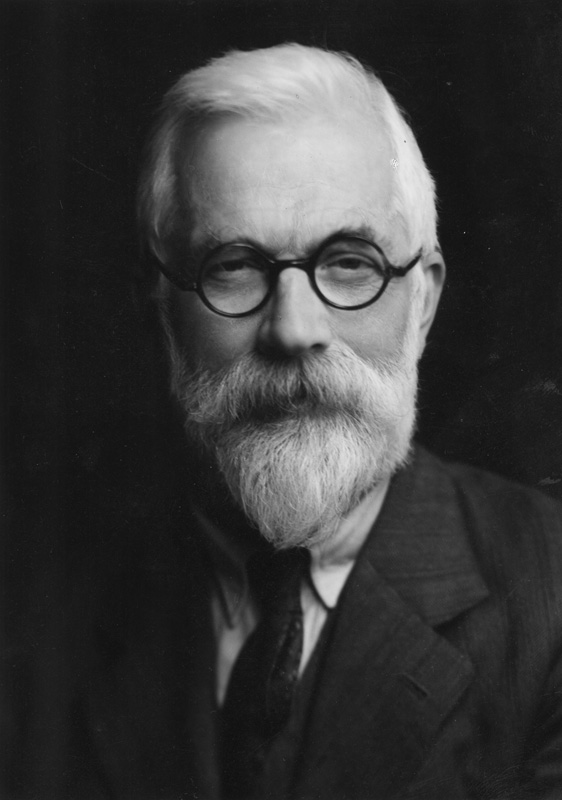
\includegraphics[width=0.5\linewidth]{R.A.Fisher.jpg}
    \caption{R. A. Fisher}
    \label{fig:Fisher}
\end{figure}
贫完之后我们闲话少叙,进入本节的正餐Fisher信息量。这是一个\textbf{理解起来比较难但是用起来很简单}的东西。
\subsection{Fisher信息量}
简单地说,信息量反映着\textbf{某个统计量}对于\textbf{参数的确定程度}的贡献。比如在上一节的德国坦克问题中,如果我们能缴获更多的德军坦克,没准就能更好地估计生产坦克的总数;但是如果我缴获的坦克是5号和10号,也并没有比8号和10号多知道多少信息,无论是使用最大似然估计还是矩估计,其实都对较小号码的坦克做了忽略。更进一步地,如果我把1到10号的坦克全部缴获,在最大似然估计的这个角度而言,实际上也和只缴获一个10号坦克没什么差别,所以我们需要一个相对确定的标准来衡量「信息」这个东西,这就引入了Fisher信息量。\par


我们应该注意,Fisher信息量是\textbf{针对于某个统计量}而言的,一般说“某某统计量(或者样本)所包含参数$\theta$的Fisher信息量”。抛开统计量谈Fisher信息量都是耍流氓,比如书上的例2.3.1,我不知道能不能像书上那么问,但我觉得对初学者更友好的提问方式或许是“求单次抽样的Fisher信息量”,至少明确了统计量是$x$或者说$x_1$。\par
那么参数的确定程度这样抽象的东西该如何反映出来呢?我猜想这很可能与Fisher本人热衷于极大似然估计有关,这里我们不妨假设统计量就是全部样本$T(x_1, \dots, x_n)$,对应地$E(T)$实际上就是似然函数(想想似然的概念),从而引出Fisher信息量的定义。\textbf{我们这里先不对什么是C-R正则族做讨论,可以简单地将其理解为一个概率分布,先直观地理解Fisher信息量的含义。}\\\par
根据极大似然估计的思想,我们希望找出似然函数的极值点。于是对对数极大似然函数$\ln L$求偏导,得到的函数其实有一个别名叫做\textbf{得分函数}(Score Function):
\begin{center}
    $S(x_1,\dots,x_n;\theta)=\sum_{i=1}^{n}\frac{\partial \ln L(x_1,\dots,x_n)}{\partial \theta}$ 
\end{center}\par
在这里我们不区分似然还是对数似然,统而称之为似然的一阶导函数。按照极大似然估计的思想,接下来我们要令这个一阶导等于零对吧?那么,其实这也可以等价地写成$E(S(X;\theta))=0$,而Fisher信息量其实就定义为\textbf{得分函数的二阶矩}:$I(\theta)=E[S(X;\theta)^2]$(严谨地定义应该是C-R正则族的得分函数的二阶矩)。这样搞有一个什么好处呢?因为方差的表达式是:
\begin{center}
    $Var(S(X;\theta))= E[S(X;\theta)^2]-[E(S(X;\theta))]^2$ 
\end{center} \par
所以实际上是有$I(\theta)=Var(S(X;\theta))$的。这是Fisher信息的第一层含义:\textbf{衡量了得分函数的方差}。\par
为避免和之后的概念混淆,在这里稍微整理一下:Fisher信息量定义为得分函数的二阶矩,在数值上也等于得分函数的方差。严谨且形式化地写应该是:
\begin{center}
    $I(\theta)=E_{\theta}\left[\frac{\partial}{\partial \theta} \ln p(x ; \theta)\right]^{2}$ 
\end{center}
这里$p(x ; \theta)$\textbf{是}C-R正则族的\textbf{概率密度函数}。(是的,对于C-R正则族我们就视而不见置若罔闻)\par

如果“积分的二阶导等于二阶导的积分”(按照书上的意思,一般情况下都相等,或者考试中也可以默认相等),则可以证明Fisher信息量的定义式等价于
\begin{center}
    $E[S(X;\theta)^2]=I(\theta)=-E[\frac{\partial^2}{\partial \theta^2} \ln p(x;\theta)]$
\end{center}

这里的证明细节并不重要,总之它为我们提供了一种\textbf{通过二阶导求解Fisher信息量}的方式。\par

所以这个式子实际上揭示了第二层含义:\textbf{对数概率密度函数在参数真实值处的负二阶导数的期望}。二阶导数,那就和曲率联系了起来,他不光衡量了极值点,还衡量了“陡峭程度”。如下图\footnote{\href{https://www.zhihu.com/question/26561604/answer/33275982}{费雪信息 (Fisher information) 的直观意义是什么?}}所示:
\begin{figure}[H]
    \centering
    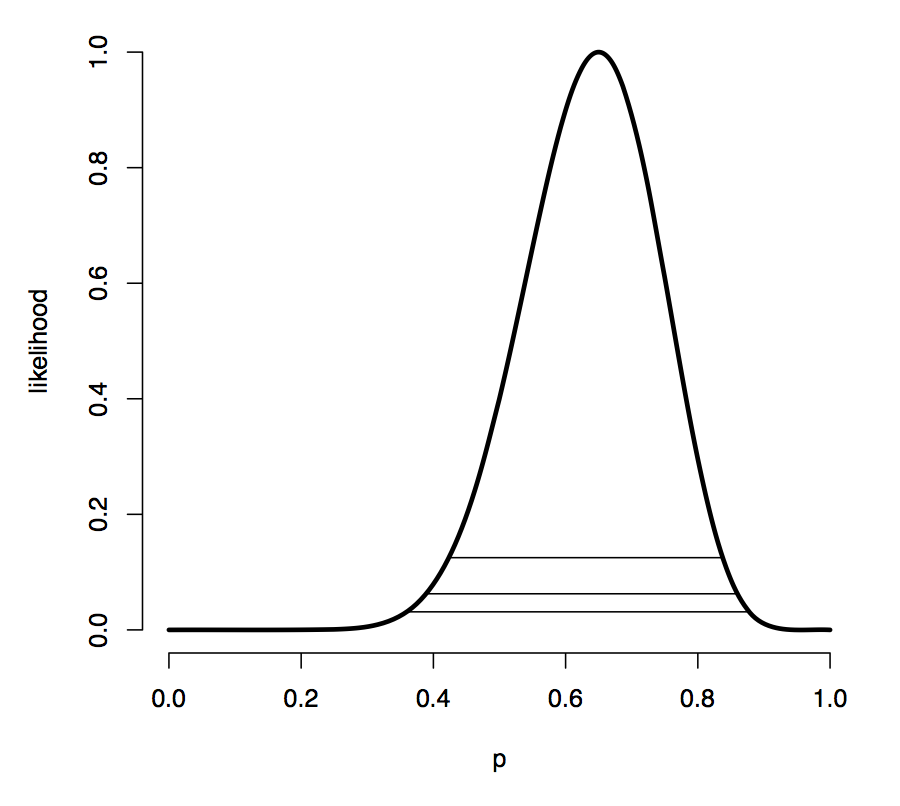
\includegraphics[width=0.8\linewidth]{likelihood.png}
    \caption{对数似然-参数 示意曲线}
    \label{fig:likelihood}
\end{figure}

我们希望这个对数似然-参数曲线越陡峭越好,这意味着参数有着更大的可能是某一值;或者说直观上看,对数似然函数这个「分布」的方差越小,即每一次观测都尽量观测到真实值,这实际上与第一个含义(得分函数的方差)联系了起来。\par
至于Fisher信息量的第三层含义,就留给下面的信息不等式说,总之,在此小结一下:
\begin{enumerate}
    \item Fisher信息量定义为C-R正则族得分函数的二阶矩。
    \item 在数值上也等于得分函数的方差。
    \item 既可以按照定义求解似然函数一阶导的二阶矩,也可以求解概率密度函数负二阶导的期望。
    \item 使用前者求解时针对于似然函数,使用后者求解时针对具体统计量。
\end{enumerate} \par
关于最后一条(或者说这两种方式的灵活使用)还需要大家结合题目去把握,目前来讲我理解得还不太充分,就不在此误人子弟了。
\subsection{信息不等式与有效估计}
还记得我们之前求解UMVUE时希望方差越小越好吗?而Fisher信息正衡量了无偏估计/充分统计量的方差,如果我们对UMVUE求Fisher信息量的话或许会得到很可观的东西,这就是信息不等式的由来。\\\par
首先介绍\textbf{Fisher信息量的可加性}。我们可以如此认为,样本越多,获得的信息量就越大,这种信息量是可加性累积的,前提是样本之间相互独立。也就是说,如果单一样本所包含的信息量是$I(\theta)$,那么n个相互独立的样本所包含的信息量就应该是$I_n(\theta)=nI(\theta)$。\par
然后我们需要\textbf{重新认识统计量}。统计量与样本有关,而抽样则是一种对信息进行压缩/提取的过程。所以统计量所包含参数$\theta$的Fisher信息$I_T(\theta)$,在直观上是\textbf{小于等于}全部样本所包含参数的Fisher信息$I_n(\theta)$的。\par
你大概可以猜到,取到等号的时候就是$T$为充分统计量的时候,这也正是所谓“充分统计量”完全反映、还原了参数信息的意义之所在,即在压缩/提取信息的过程中并没有损失。\par
当然了,请注意以上内容全部建立在C-R正则族的假设基础上,虽然这东西是啥不必知道,但如果有时候你觉得这条件也太简单了,就想想还有C-R正则族的约束就大概可以解释通了。\par
最后我们就可以给出Cramer-Rao不等式,简称C-R不等式或信息不等式(Cramer-Rao or Information Inequality),同样地这里忽略一些细微条件,给出更直观一些的定义:


\subsubsection*{Theorem 3 (信息不等式)}

$T(x_1,\dots,x_n)$是一个方差有限的统计量,令$\varphi(\theta) = E_\theta (T(x_1,\dots,x_n))$,则对于一切C-R正则族内的$\theta$,有\textbf{统计量包含参数信息}大于等于\textbf{总信息规约}后的\textbf{似然二阶矩}(在这里为平方):

\begin{center}
    $\operatorname{Var}_{\theta}\left(T\left(x_{1}, x_{2}, \cdots, x_{n}\right)\right) \geqslant \frac{\left[\varphi^{\prime}(\theta)\right]^{2}}{n I(\theta)}$
\end{center} \par
这里的证明可以从积分的定义及Cauchy-Schwarz不等式入手,有兴趣的同学可以进一步探究,在此不做展开\sout{(展开不了)}。\\\par
信息不等式揭示了一个统计量的方差下界是多少,也就是我们前边大海捞针,能将针的范围缩小到多精确。有时这个下界也被成为\textbf{Cramer-Rao下界},我们这里定义,信息不等式的右式为Cramer-Rao下界,\textbf{简称C-R下界}:$ \frac{\left[\varphi^{\prime}(\theta)\right]^{2}}{n I(\theta)}$。\par

特别地,当待估计的参数函数就是参数本身,即$\varphi(\theta) = \theta$,那么此时C-R下界退化为:$ \frac{1}{n I(\theta)}$,或者记为$ \frac{1}{I_n(\theta)}=I_n^{-1}(\theta)$,有时也直接称此为C-R下界。

由此我们便可以引出\textbf{有效估计}的概念:如果某个无偏估计$\hat q$的方差达到了C-R下界,则称其为有效估计。\par

遗憾的是,UMVUE这么伟大的东西也并不能保证其达到C-R下界,这是一个相对较强的条件。如果题目让我们论证一个无偏估计是否为有效估计,那么我们的做法就应该是求其方差,并和C-R下界对比。那么这就是一个纯数学的内容了。

\subsection{渐近无偏/有效估计}
本节内容简单地给出渐进无偏估计和渐进有效估计的概念,因为核心概念都会了,就是增加了“渐进”这一环节,所以在此不过多赘述,就总结好套路,大家结合习题练习并理解即可。

\subsubsection{渐进无偏估计}
对于$q(\theta)$的一个估计序列${T_n}$,注意这里引入了估计序列这个概念,实际上就是一个\textbf{n可变的统计量},那么如果对于一切$\theta$有:

\begin{center}
$\lim _{n \rightarrow \infty} E_{\theta}\left(T_{n}\right)=q(\theta)$    
\end{center}
则称$T_n$为$q(\theta)$的渐进无偏估计。\par
所以实际上套路可以总结为:1.求统计量期望;2.求n趋于无穷的极限,如果等于就是渐进无偏,否则不是。\par
应注意,一个有偏估计也可能是渐进无偏估计。

\subsubsection{渐进有效估计}

类似地,我们对信息不等式稍加变形,可以给出渐进有效估计的定义。同样对于$q(\theta)$的一个估计序列${T_n}$,对于一切$\theta$有:
\begin{center}
    $\lim _{n \rightarrow \infty}\left(T_{n}, q(\theta)\right)=\lim _{n \rightarrow \infty} \frac{\left[q^{\prime}(\theta)\right]^{2}}{n I(\theta)} / \operatorname{Var}_{\theta}\left(T_{n}\right)=1$    
\end{center}
则称$T_n$为$q(\theta)$的渐进有效估计。\par
所以套路也可以总结为:1.求统计量方差;2.求C-R下界;3.对二者的比值,求n趋于无穷的极限(谁在上谁在下也无所谓),如果结果等于1则为渐近有效估计,否则不是。\par
一般来说,UMVUE都是达不到C-R下界的,但一般都是一个渐进有效估计。大家可以把渐近有效估计看成对C-R估计的一种妥协,就能更好地理解这个概念了。


\end{document}